\clearpage %&latex
\documentclass[a4paper]{article}

\frenchspacing

\usepackage[cp1250]{inputenc}
\usepackage[czech]{babel}

\usepackage{a4wide}
\usepackage{amsmath, amsthm, amssymb, amsfonts}
\usepackage[mathcal]{eucal}
\usepackage{graphicx}
\usepackage{url}
\usepackage{color}
\usepackage{wrapfig}
\usepackage{capt-of}
\usepackage{float}



% sirka a vyska textu nastavena jako papir, vsechny okraje vynulovany a pridano 20pt na kazdou stranu
% horizontalni rozmery
\setlength{\textwidth}{\paperwidth}
\addtolength{\textwidth}{-40pt}
\addtolength{\hoffset}{-1in}
\addtolength{\hoffset}{20pt}
\setlength{\oddsidemargin}{0in}
\setlength{\marginparsep}{0in}
% vertikalni rozmery
\setlength{\textheight}{\paperheight}
\addtolength{\textheight}{-60pt}
\addtolength{\voffset}{-1in}
\addtolength{\voffset}{20pt}
\setlength{\topmargin}{0in}
\setlength{\headheight}{0in}
\setlength{\headsep}{0in}


%Obrazek na miste
%pouziti
%%\obrazeknahore{adresa}{popisek}{label}
\long\def\obrazeknahore#1#2#3 {

\begin{figure}[t]
    \centering
    \includegraphics[width=0.8\textwidth]{#1}
    
    \caption{#2}
    \label{#3}
    
\end{figure}

}


%==========================================
%PEKELNA MAKRA NA ZAROVNANI OBRAZKU DOPRAVA

\makeatletter


%tohle je makro, ktere mi dovoluje obtekani i u kratkych environmentu
%ABSOLUTNE nechapu, jak to funguje, ale funguje to
%viz http://tex.stackexchange.com/questions/26078/ 
\def\odrovnej{\@@par
\ifnum\@@parshape=\z@ \let\WF@pspars\@empty \fi % reset `parshape'
\global\advance\c@WF@wrappedlines-\prevgraf \prevgraf\z@
\ifnum\c@WF@wrappedlines<\tw@ \WF@finale \fi}

\makeatother



%---
%makro, co da obrazek doprava a ostatni text ho obteka
%(bez toho predchazejiciho makra to ale poradne nebeha)
%pouziti:
%\obrazekvpravo{adresa}{popisek}{label}{procento sirky}
\long\def\obrazekvpravo#1#2#3#4{

\setlength\intextsep{-20pt}

    \begin{wrapfigure}{r}{#4\textwidth}
      \begin{center}
          \vspace{-10pt}
          
        \includegraphics[width=#4\textwidth]{#1}
        \vspace{-10pt}
        
      \end{center}
      
      \caption{#2}
      \label{#3}
      
      
    \end{wrapfigure}

\setlength\intextsep{0pt}

    
}




%---
%makro pro pripady, kdy wrapfigure neco mrsi
%je to docela pekelne
%je nutne mu dat jak text vpravo, tak text vlevo
%a nevim, jestli bude 100% fungovat, ale doufam, ze jo

%pouziti:
%\obrazekvpravominipage{adresa}{popisek}{label}{procento sirky}{1 - procento sirky}{text vlevo}
\long\def\obrazekvpravominipage#1#2#3#4#5#6{

\noindent\begin{minipage}{#5\linewidth}
\vspace{0pt}
#6
\end{minipage}
\hspace{0.5cm}
\noindent\begin{minipage}{#4\linewidth}
\vspace{0pt}
\centering
\includegraphics[width=0.9\textwidth]{#1}
\captionof{figure}{#2}
\label{#3}
\end{minipage}

}

%KONEC PEKELNYCH MAKER
%=====================

% makra pro poznamku u vyrokove a predikatove logiky
\def\vl{ -- ve v�rokov� logice}
\def\pl{ -- v predik�tov� logice}


%Vacsina prostredi je dvojjazicne. V pripade, ze znenie napr pozorovania je pisane po slovensky, malo by byt po slovensky aj oznacenie.

\newenvironment{pozadavky}{\pagebreak[2]\noindent\textbf{Po�adavky}\par\noindent\leftskip 10pt}{\odrovnej\par\bigskip}
\newenvironment{poziadavky}{\pagebreak[2]\noindent\textbf{Po�iadavky}\par\noindent\leftskip 10pt}{\odrovnej\par\bigskip}


\newenvironment{definiceSkull}{\pagebreak[2]\noindent\textbf{$\bigstar$ Definice}\par\noindent\leftskip 10pt}{\odrovnej\par\bigskip}
\newenvironment{definiceNSkull}[1]{\pagebreak[2]\noindent\textbf{$\bigstar$ Definice~}\emph{(#1)}\par\noindent\leftskip 10pt}{\odrovnej\par\bigskip}

\newenvironment{definice}{\pagebreak[2]\noindent\textbf{Definice}\par\noindent\leftskip 10pt}{\odrovnej\par\bigskip}
\newenvironment{definiceN}[1]{\pagebreak[2]\noindent\textbf{Definice~}\emph{(#1)}\par\noindent\leftskip 10pt}{\odrovnej\par\bigskip}
\newenvironment{definicia}{\pagebreak[2]\noindent\textbf{Defin�cia}\par \noindent\leftskip 10pt}{\odrovnej\par\bigskip}
\newenvironment{definiciaN}[1]{\pagebreak[2]\noindent\textbf{Defin�cia~}\emph{(#1)}\par\noindent\leftskip 10pt}{\odrovnej\par\bigskip}

\newenvironment{vetaSkull}{\pagebreak[2]\noindent\textbf{$\bigstar$ V�ta}\par\noindent\leftskip 10pt}{\odrovnej\par\bigskip}
\newenvironment{vetaNSkull}[1]{\pagebreak[2]\noindent\textbf{$\bigstar$ V�ta~}\emph{(#1)}\par\noindent\leftskip 10pt}{\odrovnej\par\bigskip}

\newenvironment{pozorovani}{\pagebreak[2]\noindent\textbf{Pozorov�n�}\par\noindent\leftskip 10pt}{\odrovnej\par\bigskip}
\newenvironment{pozorovanie}{\pagebreak[2]\noindent\textbf{Pozorovanie}\par\noindent\leftskip 10pt}{\odrovnej\par\bigskip}
\newenvironment{poznamka}{\pagebreak[2]\noindent\textbf{Pozn�mka}\par\noindent\leftskip 10pt}{\odrovnej\par\bigskip}
\newenvironment{poznamkaN}[1]{\pagebreak[2]\noindent\textbf{Pozn�mka~}\emph{(#1)}\par\noindent\leftskip 10pt}{\odrovnej\par\bigskip}
\newenvironment{lemma}{\pagebreak[2]\noindent\textbf{Lemma}\par\noindent\leftskip 10pt}{\odrovnej\par\bigskip}
\newenvironment{lemmaN}[1]{\pagebreak[2]\noindent\textbf{Lemma~}\emph{(#1)}\par\noindent\leftskip 10pt}{\odrovnej\par\bigskip}
\newenvironment{veta}{\pagebreak[2]\noindent\textbf{V�ta}\par\noindent\leftskip 10pt}{\odrovnej\par\bigskip}
\newenvironment{vetaN}[1]{\pagebreak[2]\noindent\textbf{V�ta~}\emph{(#1)}\par\noindent\leftskip 10pt}{\odrovnej\par\bigskip}
\newenvironment{vetaSK}{\pagebreak[2]\noindent\textbf{Veta}\par\noindent\leftskip 10pt}{\odrovnej\par\bigskip}
\newenvironment{vetaSKN}[1]{\pagebreak[2]\noindent\textbf{Veta~}\emph{(#1)}\par\noindent\leftskip 10pt}{\odrovnej\par\bigskip}

\newenvironment{dusledek}{\pagebreak[2]\noindent\textbf{D�sledek}\par\noindent\leftskip 10pt}{\odrovnej\par\bigskip}
\newenvironment{dosledok}{\pagebreak[2]\noindent\textbf{D�sledok}\par\noindent\leftskip 10pt}{\odrovnej\par\bigskip}

\newenvironment{dokaz}{\pagebreak[2]\noindent\leftskip 10pt\textbf{D�kaz}\par\noindent\leftskip 10pt}{\odrovnej\par\bigskip}
\newenvironment{dukaz}{\pagebreak[2]\noindent\leftskip 10pt\textbf{D�kaz}\par\noindent\leftskip 10pt}{\odrovnej\par\bigskip}

\newenvironment{ideadukazu}{\pagebreak[2]\noindent\leftskip 10pt\textbf{Idea d�kazu}\par\noindent\leftskip 10pt}{\odrovnej\par\bigskip}


\newenvironment{priklad}{\pagebreak[2]\noindent\textbf{P��klad}\par\noindent\leftskip 10pt}{\odrovnej\par\bigskip}
\newenvironment{prikladN}[1]{\pagebreak[2]\noindent\textbf{P��klad~}\emph{(#1)}\par\noindent\leftskip 10pt}{\odrovnej\par\bigskip}

\newenvironment{prikladSK}{\pagebreak[2]\noindent\textbf{Pr�klad}\par\noindent\leftskip 10pt}{\odrovnej\par\bigskip}
\newenvironment{priklady}{\pagebreak[2]\noindent\textbf{P��klady}\par\noindent\leftskip 10pt}{\odrovnej\par\bigskip}
\newenvironment{prikladySK}{\pagebreak[2]\noindent\textbf{Pr�klady}\par\noindent\leftskip 10pt}{\odrovnej\par\bigskip}

\newenvironment{algoritmusN}[1]{\pagebreak[2]\noindent\textbf{Algoritmus~}\emph{(#1)}\par\noindent\leftskip 10pt}{\odrovnej\par\bigskip}
%obecne prostredie, ktore ma vyuzitie pri specialnych odstavcoch ako (uloha, algoritmus...) aby nevzniklo dalsich x prostredi
\newenvironment{obecne}[1]{\pagebreak[2]\noindent\textbf{#1}\par\noindent\leftskip 10pt}{\odrovnej\par\bigskip}

\newenvironment{report}{\pagebreak[2]\noindent\textbf{Report}\em\par\noindent\leftskip 10pt}{\par\bigskip}

%\newenvironment{reportN}[1]{\pagebreak[2]\noindent\textbf{Report~}\emph{(#1)}\emph\par\noindent\leftskip 10pt}{\odrovnej\par\bigskip}
\newenvironment{reportN}[1]{\pagebreak[2]\noindent\textbf{Report~}\emph{(#1)}\em\par\noindent\leftskip 10pt}{\odrovnej\par\bigskip}

\newenvironment{penumerate}{
\begin{enumerate}
  \setlength{\itemsep}{1pt}
  \setlength{\parskip}{0pt}
  \setlength{\parsep}{0pt}
  %\setlength{\topsep}{200pt}
  \setlength{\partopsep}{200pt}
}{\end{enumerate}}

\def\pismenka{\numberedlistdepth=2} %pouzit, ked clovek chce opismenkovany zoznam...

\newenvironment{pitemize}{
\begin{itemize}
  \setlength{\itemsep}{1pt}
  \setlength{\parskip}{0pt}
  \setlength{\parsep}{0pt}
}{\end{itemize}}

%\definecolor{gris}{gray}{0.95}
\newcommand{\ramcek}[2]{\begin{center}\fcolorbox{white}{gris}{\parbox{#1}{#2}}\end{center}\par}
 \clearpage
\title{\LARGE U�ebn� texty k st�tn� bakal��sk� zkou�ce \\ Obecn� informatika \\ Automaty a jazyky}
\begin{document}
\maketitle
\newpage
\setcounter{section}{1}
\section{Automaty a jazyky}
\begin{e}{Po�adavky}{0}{0}
\begin{pitemize}
\item Chomsk�ho hierarchie, t��dy automat� a gramatik, determinismus a nedeterminismus.
\item Uz�v�rov� vlastnosti t��d jazyk�.
\end{pitemize}
\end{e}
\def\implies{\Rightarrow}
\def\Nat{\mathbb{N}}
\def\Real{\mathbb{R}}
\def\isimplied{\Leftarrow}
\def\onlyif{\Leftrightarrow}
\def\c#1{\mathcal{#1}}


\subsection{Automaty -- Chomsk�ho hierarchie, t��dy automat� a gramatik, determinismus a nedeterminismus.}
\begin{pitemize}
\item Popi�te jednotliv� t��dy jazyk� a jejich vztahy; definujte t��dy pomoc� odpov�daj�c�ch gramatik. Napi�te priklady gramatik pro jednotliv� t��dy.

\item Popi�te automaty, ktere tyto tridv jazyku rozpozn�vaj� i  s ohledem na jejich (ne)deterministicnost.
\end{pitemize}

\subsubsection*{T��dy automat� a gramatik}

\begin{e}{Definice}{0}{Kone�n� automat}
\emph{Kone�n� automat} je p�tice $A = (Q,X,\delta,q_0,F)$, kde $Q$ je stavov� prostor (mno�ina v�ech mo�n�ch stav�), $X$ je \emph{abeceda} (mno�ina symbol�), $\delta$ je p�echodov� funkce $\delta: Q\times X\to Q$, $q_0\in Q$ je po�. stav a $F\subseteq Q$ mno�ina koncov�ch stav�.
\end{e}

\begin{e}{Definice}{0}{0}
\emph{Slovo} $w$ je posloupnost symbol� v abeced� $X$. \emph{Jazyk} $L$ je mno�ina slov, tedy $L\subseteq X^{\ast}$, kde $X^{\ast}$ je mno�ina v�ech posloupnost� symbol� abecedy $X$. $\mathbf{\lambda}$ je pr�zdn� posloupnost symbol�. \emph{Roz���en� p�echodov� funkce} je $\delta^{\ast}:Q\times X^{\ast} \to Q$ - tranzitivn� uz�v�r $\delta$. Jazyk rozpozn�van� kone�n�m automatem -- \emph{regularn� jazyk} je $L(A) = \{ w | w\in X^{\ast}, \delta^{\ast}(q_0,w)\in F \}$. \emph{Prav� kongruence} je takov� relace ekvivalence na $X^{\ast}$, �e $\forall u,v,w\in X^{\ast}: u \sim v \implies uw \sim vw$.\footnote{Pokud dv� r�zn� slova $u,v$ p�evedou automat do stejn�ho stavu (=jsou navz�jem ekvivalentn� ($u \sim v$)), pak mus� pat�it do stejn� t��dy rozkladu. Pokud k t�mto dv�ma slov�m p�id�me stejn� slovo zprava, pak tato z�et�zen� slova budou op�t pat�it do stejn� t��dy rozkladu (=mus� b�t navz�jem ekvivalentn� ($uw \sim vw$)). A toto je pr�v� ta vlastnost definuj�c� pravou kongruenci.} Je \emph{kone�n�ho indexu}, jestli�e $X^{\ast}/\sim$ (rozklad na t��dy ekvivalence) m� kone�n� po�et t��d. \begin{footnotesize}\end{footnotesize} 
\end{e}

\begin{e}{V�ta}{0}{Nerodova}
Jazyk $L$ nad kone�nou abecedou $X$ je rozpoznateln� kon. automatem $\Leftrightarrow$ existuje prav� kongruence kone�n�ho indexu $\sim$ na $X^{\ast}$ tak, �e $L$ je sjednocen�m jist�ch t��d rozkladu $X^{\ast}/\sim$.\footnote{D�le�it� tedy je, �e pokud je jazyk regul�rn�, pak pro n�j mus� existovat prav� kongruence, kter� (co� je nejd�le�it�j��) rozkl�d� v�echna slova jazyka do kone�n� mnoha t��d.}
\end{e}
\begin{e}{V�ta}{0}{Pumping (itera�n�) lemma}
Pro jazyk rozpoznateln� kon. automatem (tzn. regul�rn�) $L$ existuje $n\in \Nat$ tak, �e libovoln� slovo $z\in L,|z|\geq n$ lze ps�t jako $uvw$, kde $|uv|\leq n$, $|v|\geq 1$ a $\forall i\geq 0: uv^{i}w\in L$.\footnote{Plat� i pro kone�n� jazyky: kdy� je jazyk kone�n�, tak si za $n$ sta�� vz�t d�lku nejdel��ho slova a pak to pro v�echny slova del�� ne� n (tj. ��dn�) plat� taky. }
\end{e}

\begin{e}{Definice}{0}{0}
Dva automaty jsou \emph{ekvivalentn�}, jestli�e p�ij�maj� stejn� jazyk. \emph{Homomorfismus (isomorfismus)} automat� je zobrazen�, zachov�vaj�c� po�. stav, p�ech. funkci i konc. stavy (+ prost� a na). Pokud existuje homomorfismus automat� $A\to B$, pak jsou tyto dva ekvivalentn� (jen 1 implikace!). \emph{Dosa�iteln� stav} $q$ - $\exists w \in X^{\ast}: \delta^{\ast}(q_0,w) = q$. Relace ekvivalence je \emph{automatovou kongruenc�}, pokud zachov�v� konc. stavy a p�ech. funkci. Ke ka�d�mu automatu existuje \emph{redukt} - ekvivaletn� automat bez nedosa�iteln�ch a navz�jem ekvivalentn�ch stav�. Ten je ur�en jednozna�n� pro dan� jazyk (a� na isomorfismus), proto lze zav�st normovan� tvar.
\end{e}

\begin{e}{Pozn�mka}{0}{Operace s jazyky}
S jazyky lze prov�d�t mno�inov� operace ($\cup, \cap$), rozd�l ($\{ w | w \in L_1 \& w \notin L_2 \}$), dopln�k ($\{ w | w \notin L \}$), d�le z�et�zen� ($L_1\cdot L_2 = \{ uv | u \in L_1, v \in L_2 \}$), mocniny ($L^0={\lambda}, L^{i+1} = L^{i}\cdot L$), iterace ($L^{\ast}=L^0 \cup L^1 \cup L^2 \cup ...$), oto�en� ($L^R = \{ u^R | u\in L \}$), lev� ($L_2\setminus L_1 = \{ v | uv \in L_1, u \in L_2 \}$) i prav�
($L_1 / L_2 = \{ u | uv \in L_1, v \in L_2 \}$) kvocient $L_1$ podle $L_2$  a derivace (kvocienty podle jednoslovn�ho jazyka). T��da jazyk� rozpoznateln�ch kone�n�mi automaty je na tyto operace uzav�en�.
\end{e}

\begin{e}{Definice}{0}{Regul�rn� jazyky}
\emph{T��da regul�n�ch jazyk�} nad abecedou $X$ je nejmen�� t��da, kter� obsahuje $\emptyset$, $\forall x \in X$ obsahuje ${x}$ a je uzav�en� na sjednocen�, iteraci a z�et�zen�.
\end{e}

\begin{e}{V�ta}{0}{Kleenova}
Jazyk je regul�rn� $\Leftrightarrow$ je rozpoznateln� kone�n�m automatem.\footnote{D�kaz se d� indukc� podle po�tu hran v nedeterministick�m automatu.}
\end{e}

\begin{e}{Definice}{0}{Regul�rn� v�razy}
\emph{Regul�rn� v�razy} nad abecedou $X={x_1,...,x_n}$ jsou nejmen�� mno�ina slov v abeced� ${x_1,...,x_n,\emptyset,\lambda,^{+},\cdot,^{\ast},(,)}$, kter� obsahuje v�razy $\emptyset$ a $\lambda$ a $\forall i$ obsahuje $x_i$ a je uzav�en� na sjednocen� ($+$), z�et�zen� ($\cdot$) a iterace ($^{\ast}$). \emph{Hodnota reg. v�razu} $a$ je reg. jazyk $[a]$, lze takto reprezentovat ka�d� reg. jazyk.
\end{e}

\begin{e}{Definice}{0}{Dvoucestn� kone�n� automaty}
\emph{Dvoucestn� kone�n� automat} je p�tice $(Q,X,\delta,q_0,F)$, kde oproti kon. automatu je $\delta:Q\times X\to Q\times \{-1,0,1\}$ (tj. pohyb �tec� hlavy). P�ij�m� slovo, pokud v�po�et za�al vlevo v po�. stavu a �tec� hlava opustila slovo $w$ vpravo v konc. stavu (mimo slovo kon�� v�po�et okam�it�).
\end{e}
\begin{e}{Pozn�mka}{0}{0}
Jazyky p�ij�man� dvoucestn�mi automaty jsou regul�rn� - ka�d� dvoucestn� automat lze p�ev�st na (nedeterministick�) kone�n� automat.
\end{e}


\begin{e}{Definice}{0}{Z�sobn�kov� automaty}
\emph{Z�sobn�kov� automat} je sedmice $M=(Q,X,Y,\delta,q_0,Z_0,F)$, kde proti kone�n�m automat�m je $Y$ abeceda pro symboly na z�sobn�ku, $Z_0$ po��te�n� symbol na z�sobn�ku a funkce instrukc� $\delta:Q\times(X\cup\{\lambda\})\times Y\ \to\ \c{P}(Q\times Y^{\ast})$. Je z principu nedeterministick�; v�dy se nahrazuje vrchol z�sobn�ku, ne�te ale poka�d� vstupn� symboly. Instrukci $(p,a,Z)\to(q,w)$ lze vykonat, pokud je automat ve stavu $p$, na z�sobn�ku je $Z$ a na vstupu $a$. Vykon�n� instrukce znamen� zm�nu stavu, pokud $a\neq\lambda$, tak i posun �tec� hlavy a odebr�n� $Z$ ze z�sobn�ku, kam se vlo�� $w$ (prvn�m p�smenem nahoru). V�po�et kon�� bu� p�e�ten�m slova, nebo v p��pad�, �e pro danou situaci nen� definov�na instrukce
(\emph{Situace} z�s. automatu je trojice $(p,u,v)$, kde $p\in Q$, $u$ je nep�e�ten� zbytek slova a $v$ cel� z�sobn�k ).

P�ij�mat slovo je mo�n� bu� koncov�m stavem (slovo je p�e�teno a automat v konc. stavu), nebo z�sobn�kem (slovo je p�e�teno a z�sobn�k pr�zdn� -- konc. stavy jsou v takov�m p��pad� nezaj�mav� - $F=\emptyset$).
\end{e}

\begin{e}{Pozn�mka}{0}{0}
Pro z�s. automat p�ij�maj�c� konc. stavem v�dy existuje ekvivalentn� automat ($L(A_1)=L(A_2)$) p�ij�maj�c� z�sobn�kem a naopak.
\end{e}

\begin{e}{Definice}{0}{P�episovac� syst�m}
\emph{P�episovac� (produk�n�) syst�m} je dvojice $R=(V,P)$, kde $V$ je kone�n� abeceda a $P$ mno�ina p�episovac�ch pravidel (uspo��dan�ch dvojic prvk� z $V^{\ast}$). Slovo $w$ se \emph{p��mo p�ep�e} na $z$ ($w\Rightarrow z$), pokud $\exists u,v,x,y\in V^{\ast}: w = xuy, z = xvy, (u,v)\in P$. Derivace (\emph{odvozen�}) je z�et�zen� n�kolika p��m�ch p�eps�n�.
\end{e}

\begin{e}{Definice}{0}{Form�ln� (generativn�) gramatika}
\emph{Form�ln� gramatika} je �tve�ice $G=(V_N,V_T,S,P)$, kde $V_N$ je mno�ina netermin�ln�ch symbol� (ostatn� znaky nap�. $S$), $V_T$ mno�ina termin�ln�ch symbol�
("znaky z abecedy"), $S$ startovac� symbol ($S\in V_N$) a $P$ mno�ina pravidel. \emph{Jazyk generovan� gramatikou} je $L(G)=\{w | w\in V_T^{\ast}, S\Rightarrow^{\ast}w\}$.
\end{e}
\begin{e}{V�ta}{0}{0}
Ka�d� bezkontextov� jazyk je rozpozn�v�n z�sobn�kov�m automatem, p�ij�maj�c�m pr�zdn�m z�sobn�kem. Stejn� pro ka�d� z�sobn�kov� automat existuje bezkontextov� gramatika, kter� generuje jazyk j�m p�ij�man�.
\end{e}

\begin{e}{Pozn�mka}{0}{Vlastnosti bezkontextov�ch gramatik}
Bezkontextov� gramatika je \emph{redukovan�}, pokud $\forall X\in V_N$ existuje termin�ln� slovo $w\in V_T^{\ast}$ tak, �e $X\Rightarrow^{\ast} w$ a nav�c $\forall X\in V_N, X\neq S$ existuj� slova $u,v$ tak, �e $S\Rightarrow^{\ast}uXv$. Ke ka�d� bezkontextov� gramatice lze sestrojit ekvivalentn� redukovanou.

Pro ka�d� termin�ln� slovo v bezkontextov� gramatice existuj� derivace, kter� se li�� jen po�ad�m pou�it� pravidel (a prohozen�m n�kter�ch pravidel dostanu stejn� termin�ln� slovo), proto lze zav�st \emph{lev� (prav�) derivace} - tj. \emph{kanonick�} derivace. Pokud $X\Rightarrow^{\ast}w$, pak existuje i lev� (prav�) derivace. Zn�zorn�n� pr�b�hu derivac� je mo�n� ur�it \emph{deriva�n�m stromem} -- ur�uje jednozna�n� pravou/levou derivaci.

Bezkontextov� gramatika je \emph{v�cezna�n�} (nejednozna�n�), pokud v n� existuje slovo, kter� m� dv� r�zn� lev� derivace; jinak je \emph{jednozna�n�}. Jazyk je jednozna�n�, pokud k n�mu existuje generuj�c� jednozna�n� gramatika. Pokud je ka�d� gramatika n�jak�ho jazyka nejednozna�n�, je tento \emph{podstatn� nejednozna�n�}. 
\end{e}


\begin{e}{Definice}{0}{Greibachov� norm�ln� forma}
Gramatika je v \emph{Greibachov� norm�ln� form�}, jsou-li v�echna jej� pravidla ve tvaru $A\to au$, kde $a\in V_T$ a $u\in V_N^{\ast}$. Ke ka�d�mu bezkontextov�mu jazyku existuje gramatika v G. norm�ln� form� tak, �e $L(G)=L\setminus\{\lambda\}$. Ka�dou bezkontextovou gramatiku lze p�ev�st do G. norm�ln� formy.
\end{e}

\begin{e}{Pozn�mka}{0}{�pravy bezkontextov�ch gramatik}
Spojen�m v�ce pravidel ($A\to uBv, B\to w_1, ...B\to w_k$ se p�evede na $A\to uw_{1}v | ... | uw_{k}v$) dostanu ekvivalentn� gramatiku. Stejn� tak odstran�n�m lev� rekurze (p�evod p�es nov� netermin�l). 
\end{e}

\begin{e}{Definice}{0}{Chomsk�ho norm�ln� forma}
Pro gramatiku v \emph{Chomsk�ho norm�ln� form�} jsou v�echna pravidla tvaru $X\to YZ$ nebo $X\to a$, kde $X,Y,Z\in V_N$, $a\in V_T$. Ke ka�d�mu bezkontextov�mu jazyku $L$ existuje gramatika $G$ v Chomsk�ho norm�ln� form� tak, �e $L(G)=L\setminus\{\lambda\}$
\end{e}

\begin{e}{Pozn�mka}{0}{Vlastnosti t��dy bezkontextov�ch jazyk�}
T��da bezkontextov�ch jazyk� je uzav�en� na sjednocen�, zrcadlen�, �et�zen�, iteraci a pozitivn� iteraci, substituci a homomorfismus, inverzn� homomorfismus a kvocient s regul�rn�m jazykem. Nen� uzav�en� na pr�nik a dopln�k.
\end{e}

\begin{e}{Definice}{0}{Dyck�v jazyk}
\emph{Dyck�v jazyk} je definov�n nad abecedou ${a_1,a'_1,...a_n,a'_n}$ gramatikou $$S\to \lambda | SS | a_{1}Sa'_1 | ... | a_{n}Sa'_n$$ Je bezkontextov�, popisuje spr�vn� uz�vorkov�n� a lze j�m popisovat v�po�ty z�sobn�kov�ch automat�, tedy i bezkontextov� jazyky.
\end{e}

\begin{e}{Definice}{0}{Turing�v stroj}
\emph{Turing�v stroj} je p�tice $T=(Q,X,\delta,q_0,F)$, kde $X$ je abeceda, obsahuj�c� symbol $\varepsilon$ pro pr�zdn� pol��ko, p�echodov� funkce $\delta:(Q\setminus F)\times X\to Q\times X\times\{-1,0,1\}$ popisuje zm�nu stavu, z�pis na p�sku a posun hlavy. V�po�et kon��, nen�-li definov�na ��dn� instrukce (spec. plat� pro $q\in F$). \emph{Konfigurace} Turingova stroje jsou �daje, popisuj�c� stav v�po�tu -- nejmen�� souvisl� ��st p�sky, obsahuj�c� v�echny nepr�zdn� bu�ky a �tenou bu�ku, vnit�n� stav a poloha hlavy. \emph{Krok v�po�tu} je $uqv \vdash wpz$ pro $u$ ��st slova vlevo od akt. pozice na p�sce, $v$ od �ten�ho p�smena d�l a $q$ stav stroje. \emph{V�po�et} je posloupnost krok�, slovo $w$ je p�ij�m�no, pokud $q_{0}w \vdash^{\ast} upv$, $p\in F$. Jazyky (mno�iny slov bez $\varepsilon$) p�ij�man� Turingov�mi stroji jsou \emph{rekurzivn� spo�etn�}.
\end{e}

\begin{e}{V�ta}{0}{0}
Ka�d� jazyk typu 0 (s gramatikou s obecn�mi pravidly) je rekurzivn� spo�etn�.
\end{e}

\subsubsection*{Chomsk�ho hierarchie}
\begin{e}{Definice}{0}{Chomsk�ho hierarchie}
\emph{Chomsk�ho hierarchie} je rozd�len� gramatik do 4 t��d podle omezen� na pravidla:
\begin{figure}[!ht]
  \begin{center}
    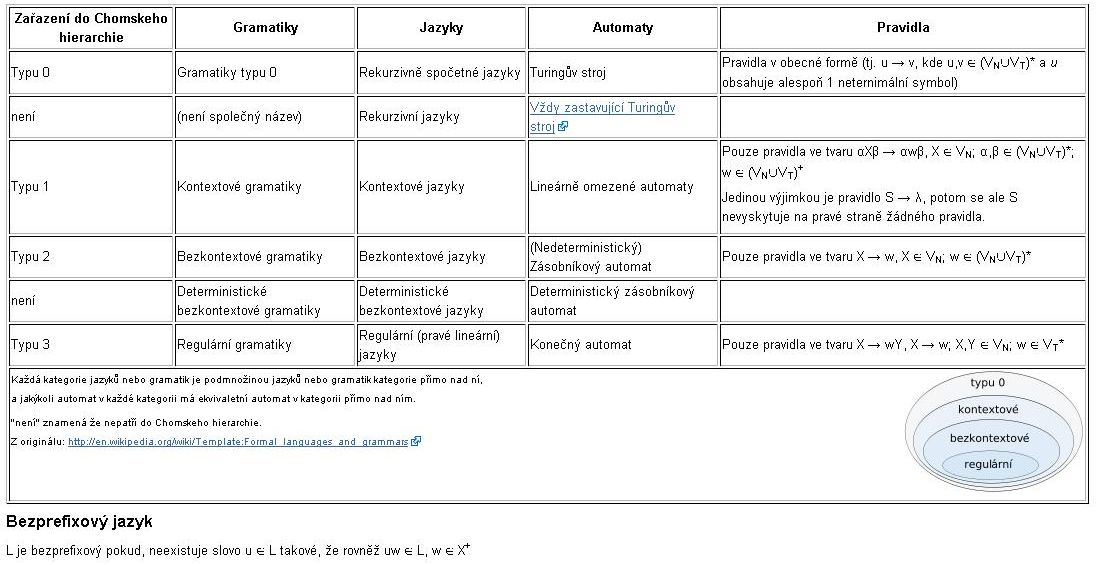
\includegraphics[scale=1.7]{informatika/teoreticka_informatika/obrazky/chomski.png}
  \end{center}
\end{figure}
\end{e}

\begin{e}{Pozn�mka}{0}{0}
S $\c{L}1 \supset \c{L}2$ nast�v� probl�m, proto�e bezkontextov� gramatiky umo��uj� pravidla tvaru $X\to\lambda$. �e�en�m je p�evod na \emph{nevypou�t�j�c� bezkontextov� gramatiky} - takov� bezkontextov� gramatiky, kter� nemaj� pravidla typu $X\to\lambda$.
\end{e}

\begin{e}{V�ta}{0}{o nevypou�t�j�c�ch bezkontextov�ch gramatik�ch}
Ke ka�d� bezkontextov� $G$ existuje nevypou�t�j�c� bezkontextov� $G_0$ tak, �e $$L(G_0)=L(G)\setminus\{\lambda\}$$ Je-li $\lambda\in L(G)$, pak $\exists G_1$, t.�. $L(G_1)=L(G)$ a jedin� pravidlo v $G_1$ s $\lambda$ na prav� stran� je $S\to\lambda$ a $S$ nen� v $G_1$ na prav� stran� ��dn�ho pravidla.
\end{e}

\begin{e}{Pozn�mka}{0}{Line�rn� gramatiky}
Pro ka�dou gramatiku typu G3 lze sestrojit kone�n� automat, kter� p�ij�m� pr�v� jazyk j� generovan�, stejn� tak pro ka�d� kone�n� automat lze sestrojit gramatiku G3. Lev� line�rn� gramatiky tak� generuj� regul�rn� jazyky, d�ky uzav�enosti na reverzi. \emph{Line�rn� gramatiky}, s pravidly typu $X\to uYv,X\to w$, kde $X,Y\in V_N, u,v,w\in V_T^{\ast}$, generuj� \emph{line�rn� jazyky} - siln�j�� ne� regul�rn� jazyky.
\end{e}

\begin{e}{Definice}{0}{Separovan� a nevypou�t�j�c� gramatika}
\emph{Separovan� gramatika} je gramatika (obecn� libovoln� t��dy), obsahuj�c� pouze pravidla tvaru $\alpha\to\beta$, kde bu� $\alpha,\beta\in V_N^+$, nebo $\alpha\in V_N$ a $\beta\in V_T\cup\{\lambda\}$. \emph{Nevypou�t�j�c� (monot�nn�) gramatika} (tak� se neomezuje na konkr�tn� t��du) je takov�, �e pro ka�d� pravidlo $u\to v$ plat� $|u|\leq|v|$.
\end{e}

\begin{e}{Pozn�mka}{0}{Kontextov� gramatiky}
Ke ka�d� kontextov� gramatice lze sestrojit ekvivalentn� separovanou. Ke ka�d� monot�nn� gramatice lze nal�zt ekvivalentn� kontextovou.
\end{e}


\subsubsection*{Determinismus a nedeterminismus}

\begin{e}{Definice}{0}{Nedeterministick� kone�n� automat}
\emph{Nedeterministick� kone�n� automat} je p�tice $(Q,X,\delta,S,F)$, kde $Q$ je mn. stav�, $X$ abeceda, $F$ mn. konc. stav�, $S$ mno�ina po��te�n�ch stav� a $\delta:Q\times X\to \c{P}(Q)$ je p�echodov� funkce. Slovo $w$ je takov�m automatem p�ij�m�no, pokud existuje posloupnost stav� $\{q_i\}_{i=1}^n$ tak, �e $q_1\in S$, $q_{i+1}\in\delta(q_i,x_i)$, $q_{n+1}\in F$.
\end{e}

\begin{e}{Pozn�mka}{0}{0}
Pro ka�d� nedeterministick� kone�n� automat $A$ lze sestrojit deterministick� kon. automat $B$ tak, �e jimi p�ij�man� jazyky jsou ekvivalentn� (m��e to znamenat exponenci�ln� n�r�st po�tu stav�).
\end{e}


\begin{e}{Definice}{0}{Deterministick� z�sobn�kov� automat}
\emph{Deterministick� z�sobn�kov� automat} je $M=(Q,X,Y,\delta,q_0,Z_0,F)$ takov�, �e $\forall p\in Q, \forall a\in (X\cup\{\lambda\}), \forall Z\in Y$ plat� $|\delta(p,a,Z)|\leq 1\footnote{definuje ze v kazdem kroku si nemuzeme vybirat}$ a nav�c pokud pro n�jak� $p, Z$ je $\delta(p,\lambda,Z)\neq\emptyset$, pak $\forall a\in X$ je $\delta(p,a,Z)=\emptyset\footnote{definuje ukon�en� vypoctu}$. 
\end{e}

\begin{e}{Pozn�mka}{0}{0}
Deterministick� z�sobn�kov� automat je \uv{slab��} ne� nedeterministick�, rozpozn�v� \emph{deterministick� bezkontextov� jazyky} koncov�m stavem a \emph{bezprefixov� bezkontextov� jazyky} pr�zdn�m z�sobn�kem (takov� jazyky, kde $u\in L(M)\implies \forall w\in X^{\ast}: uw\notin L(M)$) - kdy� se poprv� z�sobn�k automatu vypr�zdn�, v�po�et ur�it� kon��. 

Bezprefixov� bezkontextov� jazyky jsou v�dy deterministick�, opa�n� to neplat�. Deterministick� bezkontextov� jazyk lze na bezprefixov� p�ev�st z�et�zen�m s dal��m symbolem, kter� nen� v p�vodn� abeced�. 

Regul�rn� jazyky a bezprefixov� bezkontextov� jazyky jsou neporovnateln� mno�iny.
\end{e}

\begin{e}{Definice}{0}{Nedeterministick� Turing�v stroj}
\emph{Nedet. Turing�v stroj} je p�tice $T=(Q,X,\delta,q_0,F)$, kde oproti deterministick�m je $\delta:(Q\setminus F)\times X \to \c{P}(Q\times X\times \{-1,0,1\})$. P�ij�m� slovo $w$, pokud existuje n�jak� v�po�et $q_{0}w\vdash^{\ast} upv$ tak, �e $p\in F$.
\end{e}

\begin{e}{Pozn�mka}{0}{0}
Nedeterministick� Turingovy stroje p�ij�maj� pr�v� rekurzivn� spo�etn� jazyky, tj. nejsou siln�j�� ne� deterministick�. V�po�ty nedet. stroje lze toti� d�ky nekone�nosti p�sky simulovat deterministick�m (nap�. prohled�v�n�m do ���ky).
\end{e}

\begin{e}{Definice}{0}{Line�rn� omezen� automat}
\emph{Line�rn� omezen� automat} je nedeterministick� Turing�v stroj s omezenou p�skou (nap�. symboly $l$ a $r$, kter� nelze p�epsat ani se dostat mimo jejich rozmez�). Slovo je p�ij�m�no, pokud $q_{0}lwr \vdash^{\ast} upv$, kde $p\in F$. Prostor v�po�tu je omezen d�lkou vstupn�ho slova. Line�rn� omezen� automaty p�ij�maj� pr�v� kontextov� jazyky.
\end{e}


\begin{e}{Pozn�mka}{0}{Rozhodnutelnost}
Turing�v stroj m��e nep�ijmout slovo bu� skon�en�m v�po�tu v nekoncov�m stavu, nebo pokud v�po�et nikdy neskon��. Turing�v stroj \emph{rozhoduje jazyk} $L$, kdy� p�ij�m� pr�v� slova tohoto jazyka a pro libovoln� slovo je jeho v�po�et kone�n�. Takov� jazyky se naz�vaj� \emph{rekurzivn�}.

Probl�m zastaven� v�po�tu Turingova stroje je algoritmicky nerozhodnuteln� (kv�li mo�nosti jeho simulace jin�m Turingov�m strojem). Pro bezkontextov� jazyky je algoritmicky rozhodnuteln�, zda dan� slovo pat�� do jazyka. Pro bezkontextovou gramatiku nelze algoritmicky rozhodnout, zda $L(G)=X^{\ast}$. Pro dv� kontextov� gramatiky je nerozhodnuteln�, zda jejich jazyky maj� nepr�zdn� pr�nik.
\end{e}

\begin{reportN}{Hnetynka}
napisal som hierachiu, pravidla gramatik, ake automaty rozpoznavaju jednotlive gramatiky, pre reg gram veticky o KA a reg jazykoch. Pytal sa ma ako jednotlive automaty pracuju, zadal par jednoduchych prikladov a chcel zdovodnenie do akych tried patri -nakreslit/opisat slovami KA, gramatiky, ZA + dokaz pomocou pumping lemma. Pytal sa, do akej triedy by som zaradil rozpoznavanie prg jazykov, napr Java. Povedal som kontextove, ale zdovodnit som to velmi nevedel. Potvrdil ze su to kontextove + ze prave kvoli dobrym znalostam sa pouzivaju bezkontextove v kombinacii s analyzou kontextu (kedze na poradi jednotlivych riadkov zalezi) (znamka 1-2, ze zalezi na druhej inf otazke)
\end{reportN}

\begin{reportN}{Bulej}
napisal som gramatiky, odpovedajuce automaty, vysvetlil inkluzie a to bohato stacilo
\end{reportN}
\begin{reportN}{Bednarek}
M�l jsem definice hierarchie a srovn�n� s p��slu�n�mi automaty, n�stin (opravdu lehce) inkluz� mezi t��dami jazyk�, Greibachov� a Chomsk�ho n.f. plus n�jak� p��klady jazyk�, kter� dokazuj� ostrou inkluzi, ale bez p�esn�j��ch d�kaz� (kouzeln� v�ta: "to se uk�e p�es pumping lemma" ;-) ) Ptal se m� na srovn�n� deterministick�ch a nedeterministick�ch verz� jednotliv�ch druh� automat�, co� jsem v�d�l.
Informatika za jedna.
\end{reportN}
\begin{reportN}{Kucera}
Toto se obeslo bez problemu, stacilo to definovat, a rict ktere automaty prijimaij ktere jazyky, umet je definovat. Vety kolem moc zajem nevzbudily ( Nerudovka, pump. lemma):-) 
\end{reportN}
\begin{reportN}{Fiala}
Napsal sem t��dy automat�, gramatik, determinismus/nedeterminismus a pak je�t� rozhodnutelnost. P�i proch�zen� sem dost�val dopl�uj�c� ot�zky typu : "Jak n�jak l�p omezit odhad o n�rustu po�tu stavu p�i p�evodu NKA do KA" (z�le�� na po�tu po��te�n�ch stav� a na po�tu "stejnejch" p�echod� z jednotliv�ch stav�.), U rozhodnutelnosti n�znak d�kazu halting problem a dal��.
\end{reportN}
\begin{reportN}{Bedn�rek}
Tak jsem napsal automat a gramatiku ke ka�d� t��d� jazyk�, determ./nedeterm. verze a jak je to kde s jejich silou. Drobn� chyby v definic�ch nevadily, kdy� byly po upozorn�n� opraveny. U RJ se zeptal je�t� na reg. v�razy a pak taky pro� �e se rekurzivn� spo�etn� jazyky jmenuj� jak se jmenuj� (kde je ta rekurze), co� jsem nev�d�l a byl pou�en.
\end{reportN}
\begin{reportN}{IOI 10.2.2011} 
a) Popi�te jednotliv� t��dy jazyk� a jejich vztahy definujte t��dy pomoc� odpovidajicich gramatik. Napi�te p�iklady gramatik pro jednotliv� t��dy.
\\b) Popi�te automaty, ktere tyto t��dy jazyk� rozpozn�vaj� i s ohledem na jejich (ne)determinsti�nost.
\end{reportN}
\begin{reportN}{IOI 21. 6. 2011} 4.1 Popi�te Chomsk�ho hierarchii t��d jazyk�, jak se naz�vaj� jazyky v ka�d� t��d�, jak� typ gramatiky je generuje a jak� typ automatu je p�ij�m�.\\
4.2 Uve�te p��klad neregul�rn�ho jazyka a uka�te, �e nen� regul�rn�.\\
\textbf{4.3 Existuje uz�v�rov� vlastnost, na kterou nejsou uzav�en� jazyky typu 0?} TODO
\end{reportN} 
\begin{reportN}{IP 21. 6. 2011} 
Uka�te, �e n�sleduj�c� gramatika G je v�cezna�n� $S \rightarrow if\, then\, S\, else\, S\, | if\, then\, S\, | \lambda$\\
Vytvo�te gramatiku G', kter� nebude v�cezna�n�, a bude platit $L(G) = L(G')$.\\
Existuje obecn� k libovoln� bezkontextov� gramatice G jednozna�n� gramatika G' takov�, �e $L(G) = L(G')$?
\end{reportN} 


\newpage
%&latex
\subsection{Uz�v�rov� vlastnosti t��d jazyk�\footnote{Zdroj tabulky: \url{http://en.wikipedia.org/wiki/Formal_language#Operations_on_languages}}}
\begin{center}

\def\ano{\textcolor{green}{\ding{52}}}
\def\ne{\textcolor{red}{\ding{54}}}

\begin{tabular}{| p{2.4cm} | 1 | 1 | 1 | 1 | 1 | 1 | }
\hline          
    & ~RJ~ & DBKJ & ~BKJ & ~KJ~ & ~RekJ~ & ~RSJ \\          
\hline                         
Sjednocen� & \ano & \ne & \ano & \ano & \ano & \ano  \\
\hline            
  Pr�nik & \ano & \ne & \ne & \ano & \ano & \ano  \\
\hline            
  Pr�nik s RJ & \ano & \ano & \ano & \ano & \ano & \ano  \\
\hline 
  Dopln�k ($-L$) & \ano & \ano & \ne & \ano & \ano & \ne  \\
\hline 
  Homomorfismus / Substituce & \ano & \ne & \ano & \ne & \ne & \ano  \\
\hline 
  Inverzn� homo. & \ano & \ano & \ano & \ano & \ano & \ano \\
\hline
\hline  
  Zrcaden� ($L^R$) & \ano & \ne & \ano & \ano & \ano & \ano  \\
\hline  
  Z�et�zen� & \ano & \ne & \ano & \ano & \ano & \ano  \\
\hline             
  Iterace ($L^*$) & \ano & \ne & \ano & \ano & \ano & \ano  \\
\hline             
  Rozd�l  & \ano & \ne & \ne & \ano & \ano & \ano  \\
\hline  
\end{tabular}
\end{center}
Rozd�l lze vyj�d�it pomoc� pr�niku a dopl�ku tak�e z nich vypl�v�.\\
Pozor KJ nejsou uzav�en� na substituci tak jak ji definuje Bart�k\footnote{viz nap�.:
\url{http://planetmath.org/encyclopedia/RegularSubstitution.html} v tabulce
ve en-wikipedii se mluv� asi o $\lambda$-free substituci}.

\subsubsection*{Bezkontextov� jazyky}

\begin{e}{Pozn�mka}{0}{(D)BKJ nejsou uzav�en� na pr�nik}
sta�� naj�t dva BKJ, jejich� pr�nik nen� BKJ:\\
$L_1 = \{a^ib^ic^j | 0\leq i,j\} \{S\rightarrow AC, A \rightarrow aAb | \lambda, C \rightarrow cC | \lambda\}$\\
$L_2 = \{a^ib^jc^j | 0\leq i,j\} \{S\rightarrow AB, A \rightarrow aA | \lambda, B \rightarrow bBc | \lambda\}$\\
$L_1 \cap L_{2} = \{a^ib^ic^i | 0\leq i\}$ nen� BKJ (v�me z pumping lemmatu)\\
paraleln� b�h dvou z�sobn�kov�ch automat�: ��d�c� jednotky um�me spojit (viz kone�n� automaty), �ten� um�me spojit (jeden automat m��e �ekat), bohu�el dva z�sobn�ky nelze obecn� spojit do jednoho (dva z�sobn�ky = Turing�v stroj, rekurzivn� spo�etn� jazyky)
\end{e}

\begin{e}{Pozn�mka}{0}{(D)BKJ jsou uzav�en� na pr�nik s RJ}
z�sobn�kov� a kone�n� automat m��eme spojit

kone�n� automat $A_1 = (Q_1,X,\delta_1,q_1,F_1)$

z�sobn�kov� automat (p�ij�m�n� stavem) $M_2 = (Q_2,X,Y,\delta_2,q_2,Z_0,F_2)$

nov� automat $M = (Q_1 � Q_2, X, Y, \delta, (q_1,q_2), Z_0, F_1 � F_2)$

~~$((p�,q�), u) \in\delta((p,q),a,Z)$ pr�v� kdy�

~~� $a\neq\lambda: p�\in\delta_1(p,a)\ \&\ (q�,u)\in\delta_2(q,a,Z)$ � automaty �tou vstup

~~� $a=\lambda: (q�,u)\in\delta_2(q,\lambda,Z)$ � ZA m�n� z�sobn�k

~~~~~~~~~~~~~~~$p�=p$ � KA stoj�

z�ejm� $L(M) = L(A_1)\cap L(M_2)$ (paraleln� b�h automat�)
\end{e}

\begin{e}{Pozn�mka}{0}{BKJ jsou uzav�en� na sjednocen�}
pou�ijeme gramatiky (pro ZA nedeterministick� rozeskok na startu)\\
$L_1=L(G_1)$ $G_1 = (V_{N1},V_{T1},S_1,P_1)$\\
$L_2=L(G_2)$ $G_2 = (V_{N2},V_{T2},S_2,P_2)$\\
m��eme p�edpokl�dat, $�e V_{N1} \cap V_{N2} = \varnothing$ (jinak p�ejmenuj)\\
ud�l�me gramatiku:

$G = (V_{N1} \cup V_{N2} \cup \{S\}, V_{T1} \cup V_{T2}, S, P_1 \cup P_2 \cup \{S \rightarrow S_1 | S_2\})$\\
z�ejm� $L(G) = L(G_1) \cup L(G_2)$

�po��t� jedna nebo druh� gramatika
\end{e}

\begin{e}{Pozn�mka}{0}{BKJ nejsou uzav�en� na dopln�k}
sporem podle de Morganov�ch pravidel\\
$L_1 \cap L_2 = -(-L_1 \cup -L_2)$\\
bezkontextov� jazyky nejsou uzav�en� na pr�nik - SPOR\\
v ZA nesta�� prohodit koncov� a nekoncov� stavy!
\end{e}

\begin{e}{Definice}{0}{Substituce a homomorfismus}
\textit{Substituce} $\sigma$ p�ev�d� slova na jazyky

\sigma(\lambda) = \lambda, \sigma(x) = jazyk

\sigma(uv) = \sigma(u). \sigma(v) ~~\sigma: X^* \rightarrow P(Y^*)

\sigma(L) = \cup_{w\in L} \sigma(w)

T��da T jazyk� je uzav�ena na substituci, kdy�: \forall a\in X: \sigma (a)\in
T~\&~ L\in T \Rightarrow \sigma(L)\in T$
\\\\
\textit{Homomorfismus} p�ev�d� slova na slova

$h(\lambda) = \lambda, h(x) = slovo

$h(uv) = h(u) . h(v) ~~h: X^* \rightarrow Y^*

$h(L) = \{h(w) | w\in L\}$
\\\\
\textit{Inverzn� homomorfismus} p�ev�d� slova zp�t
h^{-1}(L) = \{ w | h(w)\in L\}
\end{e}

\begin{e}{Pozn�mka}{0}{BKJ jsou uzav�eny na substituci}
intuitivn�: listy v deriva�n�m stromu generuj� dal�� stromy
\\
form�ln�:
m�me bezkontextov� jazyk $L_0$, tj. gramatiku $G_0 = (V_{N0},V_{T0},S_0,P_0)$,
pro ka�d� termin�l ai z  $V_{T0}$, $\sigma(a_i)$ je bezkontextov� jazyk - gramatika $G_i$ p�edpokl�dejme, �e mno�iny netermin�l� jsou navz�jem disjunktn�
a �e ��dn� termin�l nen� v jin� gramatice netermin�lem

definujme $G = (\cup_{i\geq0}V_{Ni}, \cup_{i\geq1}V_{Ti}, S_0, P)$, kde

$P = \cup_{i\geq1}P_i \cup P'$ a $P' = P_0$, kde ka�d� termin�l $a_i$ je nahrazen $S_i$

z�ejm�: $L(G) = \sigma(L_0)$
\\
P��klad:

\begin{minipage}{0.2\linewidth}
$L_0 = \{a^ib^j ~|~ 0\leq i\leq j\}$ \\
$\sigma(a) = L_1 = {c^id^i | 0\leq i\}$ \\
$\sigma(b) = L_2 = {c^i | 0\leq i\}$ \\
$\sigma(L_0):$
\end{minipage}
\noindent\begin{minipage}{0.4\linewidth}
\vspace{0.3cm}
$S_0 \rightarrow aS_0b | S_0b | \lambda$ \\
$S1 \rightarrow cS_1d | \lambda$ \\
$S2 \rightarrow cS_2 | \lambda$ \\
$S0 \rightarrow S_1S_0S_2 | S_0S_2 | \lambda,~ S_1 \rightarrow cS_1d | \lambda,~ S_2 \rightarrow cS_2 | ?$ \\
\end{minipage}
\noindent\begin{minipage}{0.1\linewidth}
\vspace{0pt}
\centering
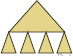
\includegraphics[width=0.9\textwidth]{informatika/teoreticka_informatika/obrazky/der_strom.png}
\end{minipage}

\end{e}

\begin{e}{Pozn�mka}{0}{BKJ jsou uzav�eny na homomorfismus}
p��m� d�sledek p�edchoz� v�ty (termin�l nahrad�me slovem)
\end{e}

\begin{e}{Pozn�mka}{0}{BKJ jsou uzav�eny na inverzn� homomorfismus}
$h^{-1}(L) = \{ w | h(w)\in L\}$ - m�me z�sobn�kov� automat M pro L a �teme w\\
idea:

� p�e�teme p�smeno x a do vnit�n�ho bufferu d�me h(x)

� simulujeme v�po�et M, kdy vstup bereme z bufferu

� po vypr�zdn�n� bufferu na�teme dal�� p�smeno ze vstupu

� slovo je p�ijato, kdy� je buffer pr�zdn� a M je v koncov�m stavu
\\
form�ln�:

buffer je kone�n�, m��eme ho tedy modelovat ve stavu
pro $L$ m�me $M = (Q,X,Y,\delta,q_0,Z_0,F)$ (p��j�m�n� koncov�m stavem)

$h: A^* \rightarrow X^*$

definujme $M' = (Q', A, Y, \delta',[q_0,\lambda], Z_0, F�\{\lambda\})$, kde

$Q' = \{[q,u] ~|~ q\in Q,~ u\in X^*, ~\exists a\in A ~\exists v\in X^* ~h(a)=vu\}$, u je buffer

$\delta'([q,u], \lambda, Z) = \{ ([p,u],\gamma) | (p,\gamma) \in \delta(q, \lambda, Z) \}$

~~~~~~~~~~~~~~~~~~$\cup~ \{ ([p,v],\gamma ) ~|~ (p,\gamma) \in (q, b, Z) \}$ � $u=bv$ (�te buffer)

$\delta'([q, \lambda], a, Z) = \{ ([q,h(a)],Z) \}$ � napl�uje buffer
\end{e}

\begin{e}{Pozn�mka}{0}{DBKJ nejsou uzav�en� na sjednocen� (BKJ ano)!}
P��klad:

$L = {a^ib^jc^k ~|~ i\neq j ~OR~ j\neq k ~OR~ i\neq k\}$ je BKJ, ale nen� DBKJ

sporem: nech� $L$ je DBKJ
potom $-L$ (dopln�k) je DBKJ

$-L \cap a*b*c* = \{a^ib^jc^k | i=j=k\}$ je DBKJ - SPOR
\end{e}

\begin{e}{Pozn�mka}{0}{DBKJ nejsou uzav�en� na homomorfismus (BKJ ano)!}
P��klad:

$L_1 = \{a^ib^jc^k | i=j\}$ je DBKJ

$L_2 = \{a^ib^jc^k | j=k\}$ je DBKJ

$0L_1 \cup 1L_2$ je DBKJ, $1L_1 \cup 1L_2$ nen� DBKJ

polo�me $h(0) = 1$ a $h(x) = x$ pro ostatn� symboly

$h(0L_1 \cup 1L_2) = 1L_1 \cup 1L_2$
\end{e}



\begin{e}{Pozn�mka}{0}{Dopln�k deterministick�ho BKJ je op�t deterministick� BKJ!}
prohod�me koncov� a nekoncov� stavy\\
pot�e:\\
� nemus� p�e��st cel� vstupn� slovo\\
� krok nen� definov�n (nap�. vypr�zdn�n� z�sobn�ku)

snadno o�et��me �podlo�kou� na z�sobn�ku\\
� cyklus (z�sobn�k roste, z�sobn�k pulsuje)

odhal�me pomoc� ��ta�e\\
� po p�e�ten� slova proch�z� koncov� a nekoncov� stavy

sta�� si pamatovat, zda pro�el koncov�m stavem
\end{e}

\subsubsection*{Kontextov� jazyky}

\begin{e}{Pozn�mka\footnote{J.Hopcroft,J.Ullmann: FORMAL LANGUAGES AND THEIR RELATION TO AUTOMATA, str.127}}{0}{KJ nejsou uzav�en� na substituci a homomorfismus}
Proof Let $G_1 = (V_N, V_T, P_1, S)$ be a type 0 grammar such that $L(G_1)$ is
not a context-sensitive language. We assume without loss of
generality that the productions are of the form $\alpha\rightarrow\beta$ or $A\rightarrow a$, where $\alpha\in V^+_N$, $\beta \in V^*_N$, $A \in V_N$, and $a \in V_T$. Let $c$ be a new symbol.
\\Consider the grammar $G_2 = (V_N, V_T\cup \{C\}, P_2, S)$ where $P_2$ contains:
\\1. $\alpha\rightarrow\beta$ if $\alpha\rightarrow\beta$ is in $P_2$ and $|\alpha|\leq|\beta|$.
\\2. $\alpha\rightarrow\beta cc...c$ where $|\alpha|=|\beta cc...c|$ if $\alpha\rightarrow\beta$ is in $P_2$ and $|\alpha|<|\beta|$.
\\3. $cA\rightarrow Ac$ $\forall A \in V_N$.
\\The grammar $G_2$ is context sensitive, since we have forced the right-hand
side of every Production to be at least as long as the left-hand side. The
productions $cA\rightarrow Ac$ were added to move the $c$'s to the right end of
the words so that derivations in $G_2$ can proceed as in $G_1$. Now consider the
substitution
\\$\sigma(a) = \{a\}$ for $a \in V_T$ and $\sigma(c) = \{\lambda\}$.
\\Then $\sigma(L(G_2)) = L(G_1)$ (a type 0 grammar) and hence substitution does not preserve the class
of Context-sensitive languages.
\\\\ \LARGE\sun\normalsize~ The substitution used in the proof is a homomorphism.
\end{e}

\subsubsection*{Rekurzivn� a rekurzivn� spo�etn� jazyky}

\begin{e}{V�ta}{0}{Postova}
$L$ je rekurzivn� $\Leftrightarrow$ $-L$ a $L$ jsou rekurzivn� spo�etn�
\end{e}

\begin{e}{Pozn�mka\footnote{Zdroj: \url{http://youbo2010.blogspot.com/2011/04/why-recursive-languages-are-not-closed.html}}}{0}{RSJ
jsou a RekJ nejsou uzav�en� na homomorfismus}
First let's consider a much simpler problem, inverse homomorphism, in which w is in L' if and only h(w) is in L. We can just apply h to w and let the TM accepting L run with input h(w). So L' is recursively enumerable(resp. recursive) if L is recursively enumerable(resp. recursive).
\\\\
Now we'll attack homomorphism, in which $x\in L' \Leftrightarrow \exists
w\in L : h(w)=x$.
\\\\
For recursively enumerable languages, the slide say that we can design an NTM M to take as input $x$, guess an $w$ such that $h(w)=x$ and simulate $M_1$ on $w$ (suppose $L=L(M_1)$). I will give a detailed sketch on how $M$ behaves. It

0) sets $l$ to 1

1) guesses one $w$ of length $l$

2) if there is such an $w$ invokes $M_1$ otherwise goes to 4)

3) if $M_1$ accepts so would M otherwise goes to 4)

4) increases $l$ by 1 and goes back to 1)
\\\\
So if $L$ is recursively enumerable, so is $L'$.
And of course we can use a DTM that generates each $w$ in a systematic way.
\\\\
Now what about recursive languages? Even though $L$ is recursive, the above process may not halt since there may be infinitely many $w$'s such that $h(w)=x$ but none of these $w$'s is in $L$. A automat $M$ se prost� zacykl�.
\\\\
To show recursive languages not closed under homomorphism, consider
the language $L=\{<M,w, a^i> |$ TM M accepts w in i steps$\}$, which is recursive.
However, if a homomorphism h maps a to $\lambda$ while keeping the remaining symbols intact, $h(L)=\{<M,w> |$ TM M accepts w$\}$ which is not recursive.\footnote{http://www.cs.uiuc.edu/class/fa10/cs373/lectures/lect18.pdf}
\end{e}

\begin{e}{Pozn�mka}{0}{Dopln�k RekJ mus� v�dy b�t RekJ}
Nech� jazyk L je rekurzivn�. Pak jist� existuje TS M, kter� tento jazyk rozhoduje. Tento TS M pracuje tak, �e v�echna slova w z L p�ijme a v�echna slova z -L (= dopln�k jazyka L) odm�tne. Nov� TS M', kter� bude rozhodovat jazyk -L sestroj�me takto:

    $\bullet$ Simuluj �innost TS M pro vstup w.

    $\bullet$ Pokud TS M slovo p�ijme, odm�tni. Pokud TS M slovo odm�tne, p�ijmi.
\\
Nov� TS M' bude jednodu�e vracet p�esn� opa�n� v�sledky, ne� p�vodn� TS M. Tento TS M' rozhoduje jazyk -L.
\end{e}

\begin{e}{Pozn�mka}{0}{Dopln�k RSJ nemus� v�dy b�t RSJ}
Komplementem �ist� RSJ (tedy jazyka, kter� je RSJ, ale nen� rekurzivn�) je v�dy jazyk, kter� nen� rekurzivn� spo�etn�. Vezm�me pro p��klad jazyk HALT, kter� je �ist� RSJ, ale jeho komplement (NotHALT) nen� RSJ. To vypl�v� z definice NotHALT: HALT obsahuje dvojice TS:slovo takov�, �e TS pro dan� slovo zastav�. NotHALT tedy obsahuje dvojice TS:slovo takov�, kdy dan� TS nezastav� pro slovo, �e se zacykl�. Proto�e nejsme schopni identifikovat cyklus, nejsme schopni sestavit TS, kter� by jazyk NotHALT p�ij�mal. Obecn�: pokud m�me jazyk L, kter� je �ist� RSJ, pak jeho komplement -L mus� obsahovat takov� slovo, pro n� se TS M' zacykl� a tud� tento TS M' nem��e p�ij�mat jazyk -L.
\end{e}

TODO: nejaka zduvodneni chyb�



\end{document}
